\clearpage
\subsection{$\boldsymbol{\mathrm{LiFePO}_4}$ battery model} \label{sec_bat_res}
As already mentioned, the Offgridtec Smart-Pro $12,8\mathrm{V}$ $50\mathrm{Ah}$ $\mathrm{LiFePO_4}$ battery -- which from now on will simply be refered to as battery -- is used to store the electrical energy converted by the PV generator and to supply the repeater radio infrastructure with it. Table \ref{tab:table_smart_pro_lifepo4_battery} contains an excerpt from the data sheet for this battery, with which the nominal current of the battery can be calculated using the equation (\ref{eq:i_nom}) to $I_\mathrm{nom} = 16,67\mathrm{A}$. 
\begin{table}[h!]
	\centering
	\footnotesize
\begin{tabular}{|l|c|}
	\hline
	\multicolumn{2}{|c|}{\textbf{Offgridtec Smart-Pro $\boldsymbol{12,8\mathrm{V}}$ $\boldsymbol{50\mathrm{Ah}}$ specifications}} \\
	\hline
	Nominal charge for $\mathrm{C_D} = 1/3\mathrm{h}^{-1}$ & $50\mathrm{Ah}$ \\
	Nominal discharging current & $16,7\mathrm{A}$ \\
	Nominal voltage & $12,8\mathrm{V}$ \\
	Working voltage & $11,0\mathrm{V}$ to $14,6\mathrm{V}$ \\
	Maximum continuous discharging current & $50\mathrm{A}$ \\
	Recommended continuous discharging current & $20\mathrm{A}$ \\
	Maximum charging current & $50\mathrm{A}$ \\
	Recommended charging current & $25\mathrm{A}$ \\
	Maximum charging voltage & $14,4\pm0,2\mathrm{V}$ \\
	Float charge voltage & $13,8\pm0,2\mathrm{V}$ \\
	Minimum number of cycles & $>2500$ \\
	\hline
	Charging temperature & $-20^\circ\mathrm{C}$ to $60^\circ\mathrm{C}$ \\
	Discharging temperature & $-5^\circ\mathrm{C}$ to $45^\circ\mathrm{C}$ \\
	Storage temperature ($20\%$ to $75\%$ humidity) & $0^\circ\mathrm{C}$ to $20^\circ\mathrm{C}$ \\
	\hline
	BMS & Integrated \\
	Bluetooth & Integrated \\
	\hline
\end{tabular}
	\caption{Excerpt from the data sheet of the Offgridtec Smart-Pro $12,8\mathrm{V}$ $50\mathrm{Ah}$ $\mathrm{LiFePO_4}$ battery \cite{Offgridtec:2020}.}
	\label{tab:table_smart_pro_lifepo4_battery}
\end{table}

So that this battery can be used with the \MATLAB simulation in the appendix \ref{sec:matlab_code}, the discharging and charging experiments discussed in the subsection \ref{sec:electrochemical} had to be carried out. The laboratory equipment required for these experiments is listed in the table \ref{tab:table_dis_chrg_exp_equipm}.
\begin{table}[h!]
	\centering
	\footnotesize
\begin{tabular}{|l|c|}
	\hline
	\multicolumn{2}{|c|}{\textbf{Laboratory equipment}} \\
	\hline
	Oscilloscope & Keysight DSOX 1102G \\
	Shunt resistor & Lumel $60\mathrm{mV}$ $50\mathrm{A}$ ($1,2\mathrm{m}\Omega$) \\
	Electronic load & FTVOGUE17cm0w5uh2 \\
	Battery charger & Mean Well ENC-180-12 \\
	\hline
\end{tabular}
	\caption{Laboratory equipment required to carry out the discharging and charging experiment with the Offgridtec Smart-Pro $12,8\mathrm{V}$ $50\mathrm{Ah}$ $\mathrm{LiFePO_4}$ battery.}
	\label{tab:table_dis_chrg_exp_equipm}
\end{table}
A total of four electronic loads connected in parallel were used. This was done because each electronic load could only convert a maximum power of $60\mathrm{W}$ into heat. To assure that these were switched on and off at the same time, a central button for all electronic loads was used.

Before the experiments were carried out, the internal resistances of the input channels 1 and 2 of the oscilloscope were measured. These measurements resulted in $R_\mathrm{Ch1} = 1011,68\mathrm{k}\Omega$ for Ch1 and $R_\mathrm{Ch2} = 1004,99\mathrm{k}\Omega$ for Ch2. Taking into account the battery voltage $U_\mathrm{B}$ for the upper left and the current divider rule for the upper right loop in the figures \ref{fig:tikz_experiment_1} and \ref{fig:tikz_experiment_2}, it was determined that the resulting currents $I_\mathrm{Ch1}$ and $I_\mathrm{Ch2}$ are negligibly small. This applies because during the discharging experiment $I_\mathrm{L}$ was set so that $I_\mathrm{D}$ is equal to $I_\mathrm{nom}$ and during the charging experiment the battery charger provides a current of $I_\mathrm{BC} = 12\mathrm{A}$ \cite{MeanWell}. It is noted that neglecting $I_\mathrm{Ch1}$ and $I_\mathrm{Ch2}$ has the consequence that $I_\mathrm{D} = I_\mathrm{L}$ and $I_\mathrm{C} = I_\mathrm{BC}$.

Both experiments were carried out in such a way that measuring points were recorded in $0,05$ steps of the SOC. Thus, $N_\mathrm{MP} = 21$ measuring points had to be recorded per experiment. Based on this -- while taking into account the equation (\ref{eq:battery_charge}) and that $\eta_\mathrm{C} = 1$ -- the equations (\ref{eq:delta_t_D}) and (\ref{eq:delta_t_C}) result in $\Delta t_\mathrm{D} = 8,98\mathrm{min}$ and $\Delta t_\mathrm{C} = 12,5\mathrm{min}$. Since the battery has integrated Bluetooth, its SOC was additionally observed -- in parallel to a set timer -- using the Offgridtec Battery Viewer Smart Android app provided by Offgridtec GmbH.  
 
In order to get to the next measuring point, the battery had to be discharged with $I_\mathrm{D}$ over the time interval $\Delta t_\mathrm{D}$ or charged with $I_\mathrm{C}$ over the time interval $\Delta t_\mathrm{C}$. When this measuring point was reached, the currents were switched off. After 20min it could be clearly observed with Ch1 of the oscilloscope that the battery voltage hardly changed. Therefore $t_\mathrm{rest}$ was set to this time. At each measuring point the ambient temperature $\vartheta_\mathrm{A}$ was measured with a Newentor weather station (ASIN: B08M6C4MCM). This resulted in a \emph{mean ambient temperature} during the discharging experiment of $\overline{\vartheta}_\mathrm{A,D} = 23,99^\circ\mathrm{C}$ and during the charging experiment of $\overline{\vartheta}_\mathrm{A,C} = 25,23^\circ\mathrm{C}$.

Two recorded measurements for the discharging and charging experiment for $\mathrm{SOC}_n = 0,5$ can be seen in the figures \ref{fig:image_dis_50} and \ref{fig:image_chg_50}. The blue y-axes represent Ch1 and the green y-axes represent Ch2 of the oscilloscope. The green continuous lines are the currents $I_\mathrm{D}(t)$ and $I_\mathrm{C}(t)$ and the blue continuous lines are the battery voltages $U_\mathrm{B}(t)$ for the respective experiments. Furthermore, several cursors can be seen. In the case of the currents $I_\mathrm{D}(t)$ and $I_\mathrm{C}(t)$, the green dash-dotted cursor indicates their top value, and the green dashed cursor indicates their bottom value. In the case of the battery voltages $U_\mathrm{B}(t)$, the blue cursors mark the voltage drop for both experiments. The voltage drop instead of the voltage rise was used for the charging experiment because the observed rising slope was not steep enough -- after switching on $I_\mathrm{C}(t)$. This could falsify the result for calculating the electrolyte resistance $R_\mathrm{e,C}(\mathrm{SOC}_n)$. Similar to the currents, the blue dash-dotted cursor represents the top value of the voltage drop and the blue dashed cursor the bottom value of the voltage drop. 
\begin{figure}[h!]
	\centering
  	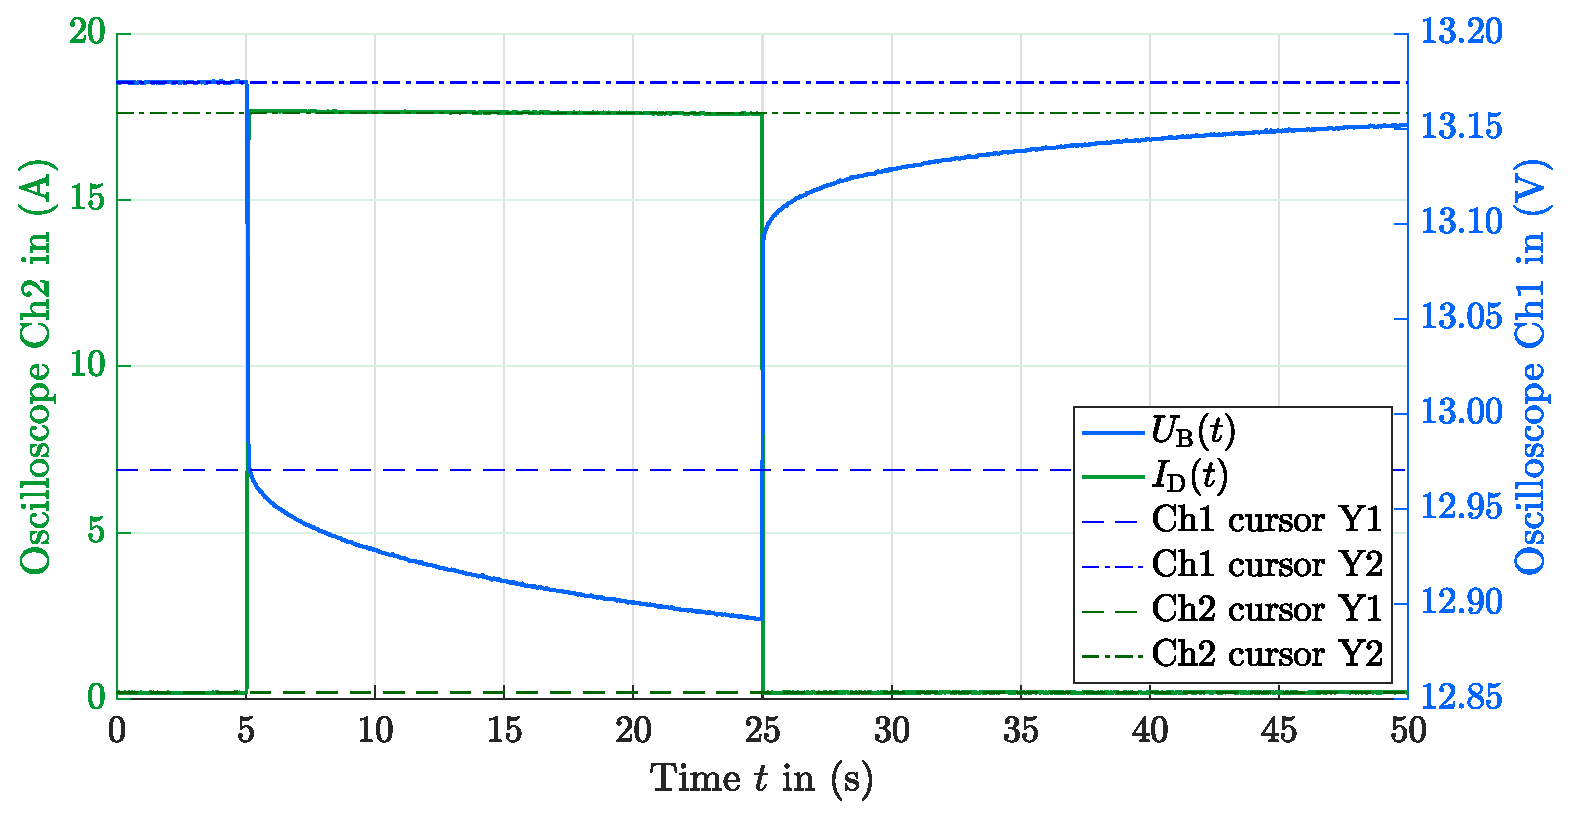
\includegraphics[width = 0.9\textwidth]{image_dis_50.eps}
  	\caption{Recorded time courses of $U_\mathrm{B}(t)$ and $I_\mathrm{D}(t)$ during the discharging experiment for $\mathrm{SOC}_n = 0,50$. The device under test was the Offgridtec Smart-Pro $12,8\mathrm{V}$ $50\mathrm{Ah}$ $\mathrm{LiFePO_4}$ battery.}
	\label{fig:image_dis_50}
\end{figure}
\begin{figure}[h!]
	\centering
  	\includegraphics[width = 0.9\textwidth]{image_chg_50.eps}
	\caption{Recorded time courses of $U_\mathrm{B}(t)$ and $I_\mathrm{C}(t)$ during the charging experiment for $\mathrm{SOC}_n = 0,50$. The device under test was the Offgridtec Smart-Pro $12,8\mathrm{V}$ $50\mathrm{Ah}$ $\mathrm{LiFePO_4}$ battery.}
	\label{fig:image_chg_50}
\end{figure}

The time courses of the channels 1 and 2 shown in the figures \ref{fig:image_dis_50} and \ref{fig:image_chg_50} were recorded with the oscilloscope for all measuring points, with each being saved in a seperate\codeword{.cvs}file. Subsequently, the data in the\codeword{.cvs}files were processed with a \MATLAB program, in which the function\codeword{ischange()}was used to determine the positions of the cursors. The currents $I_\mathrm{D}(\mathrm{SOC}_n)$ and $I_\mathrm{C}(\mathrm{SOC}_n)$ as well as the voltage drops $\Delta U_\mathrm{D}(\mathrm{SOC}_n)$ and $\Delta U_\mathrm{C}(\mathrm{SOC}_n)$ were then calculated by subtracting their respective dashed cursor from their dash-dotted cursor. Now that all the required parameters were known, the electrolyte resistances $R_\mathrm{e,D}(\mathrm{SOC}_n)$ and $R_\mathrm{e,C}(\mathrm{SOC}_n)$ were determined using the equations (\ref{eq:r_0_d_soc}) and (\ref{eq:r_0_c_soc}).

For completeness it must be mentioned that the scales of the green y-axes from the figures \ref{fig:image_dis_50} and \ref{fig:image_chg_50} were calculated with this \MATLAB program by extracting the Ch2 data -- which represents the measured voltage drop across the shunt resistor -- from the\codeword{.cvs}files and applying it to the equations (\ref{eq_i_d_real}) and (\ref{eq:i_c_real}).

It should further be noted that $\Delta t_\mathrm{D}$ and $\Delta t_\mathrm{C}$ cannot be seen in the figures \ref{fig:image_dis_50} and \ref{fig:image_chg_50}, since these are the time intervals between two successive measuring points. The time interval between switching the discharging or charging current on and off -- for a certain measuring point -- was determined during the course of the experiments. When $t_\mathrm{rest}$ was over, the open-circuit voltages $U_\mathrm{0,D}(\mathrm{SOC}_n)$ and $U_\mathrm{0,C}(\mathrm{SOC}_n)$ were measured, the time scale of the oscilloscope was set to 50s and Ch1 was triggered manually. After approximately 5s, either the electronic load or the charger was switched on manually. After another 20s these were switched off again. This approach gave the best results. From the measured open-circuit voltages, $U_\mathrm{0}(\mathrm{SOC}_n)$ was calculated with the equation (\ref{eq:U_0}).

The results of the experiments are summarized in the table \ref{tab:table_exp_results} and visualized in the figures \ref{fig:image_open_circuit_voltages_matlab} and \ref{fig:image_electrolyte_resistances_matlab}. To obtain the battery model, these now only have to be interpolated and inserted into the equation (\ref{eq:battery_voltage_adapted}). 
\begin{table}[h!]
	\centering
	\footnotesize
\begin{tabular}{|c|c|c|c|c|c|}
	\hline
	$\boldsymbol{\mathrm{SOC}_n}$ & $\boldsymbol{R_\mathrm{e,D}(\mathrm{SOC}_n)}$ & $\boldsymbol{R_\mathrm{e,C}(\mathrm{SOC}_n)}$ & $\boldsymbol{U_\mathrm{0,D}(\mathrm{SOC}_n)}$ & $\boldsymbol{U_\mathrm{0,C}(\mathrm{SOC}_n)}$ & $\boldsymbol{U_\mathrm{0}(\mathrm{SOC}_n)}$ \\
	\hline
1,00 & $0,0121\Omega$ & $0,0121\Omega$ & $13,877\mathrm{V}$ & $14,107\mathrm{V}$ & $13,9920\mathrm{V}$\\ 
0,95 & $0,0117\Omega$ & $0,0113\Omega$ & $13,315\mathrm{V}$ & $13,387\mathrm{V}$ & $13,3510\mathrm{V}$\\ 
0,90 & $0,0118\Omega$ & $0,0115\Omega$ & $13,319\mathrm{V}$ & $13,393\mathrm{V}$ & $13,3560\mathrm{V}$\\ 
0,85 & $0,0117\Omega$ & $0,0114\Omega$ & $13,322\mathrm{V}$ & $13,401\mathrm{V}$ & $13,3615\mathrm{V}$\\ 
0,80 & $0,0116\Omega$ & $0,0115\Omega$ & $13,320\mathrm{V}$ & $13,415\mathrm{V}$ & $13,3675\mathrm{V}$\\ 
0,75 & $0,0116\Omega$ & $0,0116\Omega$ & $13,306\mathrm{V}$ & $13,388\mathrm{V}$ & $13,3470\mathrm{V}$\\ 
0,70 & $0,0117\Omega$ & $0,0112\Omega$ & $13,248\mathrm{V}$ & $13,387\mathrm{V}$ & $13,3175\mathrm{V}$\\ 
0,65 & $0,0116\Omega$ & $0,0112\Omega$ & $13,196\mathrm{V}$ & $13,275\mathrm{V}$ & $13,2355\mathrm{V}$\\ 
0,60 & $0,0116\Omega$ & $0,0111\Omega$ & $13,181\mathrm{V}$ & $13,272\mathrm{V}$ & $13,2265\mathrm{V}$\\ 
0,55 & $0,0117\Omega$ & $0,0112\Omega$ & $13,117\mathrm{V}$ & $13,253\mathrm{V}$ & $13,1850\mathrm{V}$\\ 
0,50 & $0,0117\Omega$ & $0,0113\Omega$ & $13,174\mathrm{V}$ & $13,250\mathrm{V}$ & $13,2120\mathrm{V}$\\ 
0,45 & $0,0117\Omega$ & $0,0113\Omega$ & $13,172\mathrm{V}$ & $13,248\mathrm{V}$ & $13,2100\mathrm{V}$\\ 
0,40 & $0,0118\Omega$ & $0,0114\Omega$ & $13,169\mathrm{V}$ & $13,250\mathrm{V}$ & $13,2095\mathrm{V}$\\ 
0,35 & $0,0118\Omega$ & $0,0115\Omega$ & $13,111\mathrm{V}$ & $13,244\mathrm{V}$ & $13,1775\mathrm{V}$\\ 
0,30 & $0,0118\Omega$ & $0,0114\Omega$ & $13,087\mathrm{V}$ & $13,225\mathrm{V}$ & $13,1560\mathrm{V}$\\ 
0,25 & $0,0118\Omega$ & $0,0115\Omega$ & $13,012\mathrm{V}$ & $13,179\mathrm{V}$ & $13,0955\mathrm{V}$\\ 
0,20 & $0,0118\Omega$ & $0,0116\Omega$ & $12,931\mathrm{V}$ & $13,089\mathrm{V}$ & $13,0100\mathrm{V}$\\ 
0,15 & $0,0118\Omega$ & $0,0115\Omega$ & $12,837\mathrm{V}$ & $12,958\mathrm{V}$ & $12,8975\mathrm{V}$\\ 
0,10 & $0,0117\Omega$ & $0,0117\Omega$ & $12,814\mathrm{V}$ & $12,923\mathrm{V}$ & $12,8685\mathrm{V}$\\ 
0,05 & $0,0118\Omega$ & $0,0118\Omega$ & $12,350\mathrm{V}$ & $12,502\mathrm{V}$ & $12,4260\mathrm{V}$\\ 
0,00 & $0,0121\Omega$ & $0,0121\Omega$ & $11,371\mathrm{V}$ & $11,420\mathrm{V}$ & $11,3955\mathrm{V}$\\
	\hline
\end{tabular}
	\caption{Calculated results from the discharging and charging experiment carried out on the Offgridtec Smart-Pro $12,8\mathrm{V}$ $50\mathrm{Ah}$ $\mathrm{LiFePO_4}$ battery.}
	\label{tab:table_exp_results}
\end{table}
\begin{figure}[h!]
	\centering
  	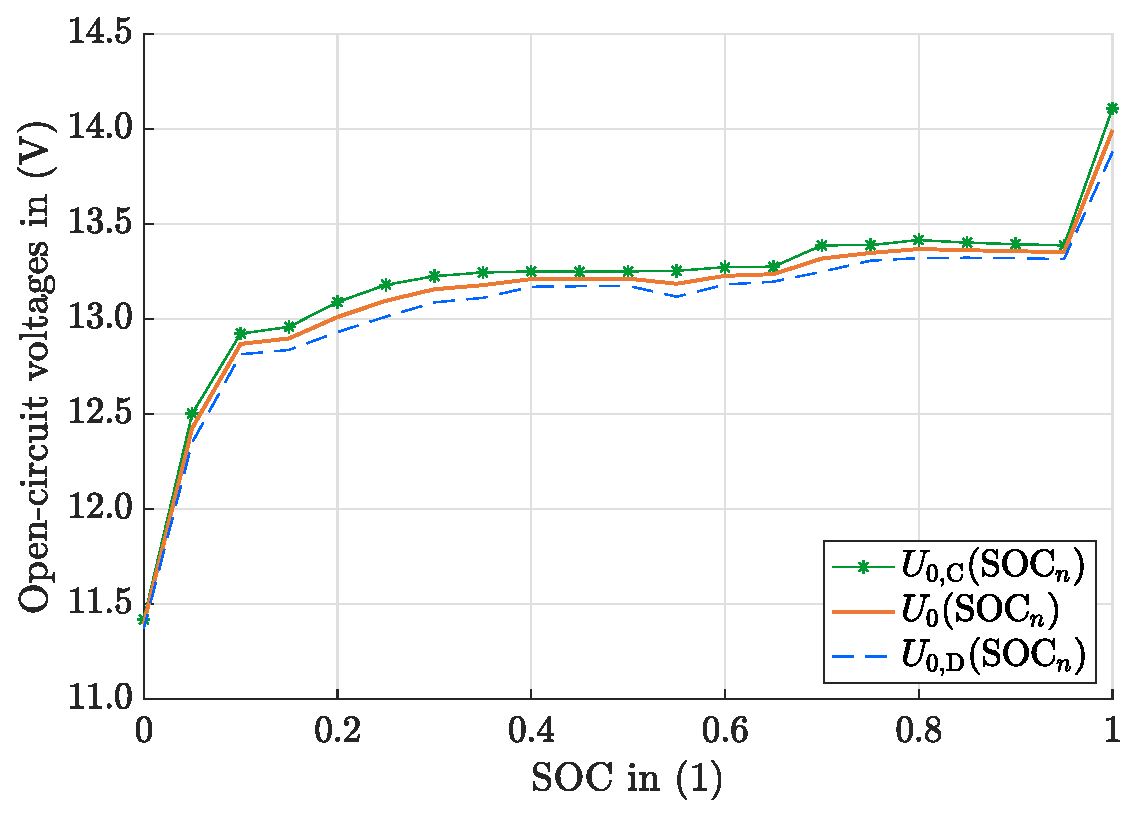
\includegraphics[width = 0.67\textwidth]{image_open_circuit_voltages_matlab.eps}
  	\caption{Open-circuit voltages $U_\mathrm{0,C}(\mathrm{SOC}_n)$, $U_\mathrm{0}(\mathrm{SOC}_n)$ and $U_\mathrm{0,D}(\mathrm{SOC}_n)$ obtained from the discharging and charging experiment carried out on the Offgridtec Smart-Pro $12,8\mathrm{V}$ $50\mathrm{Ah}$ $\mathrm{LiFePO_4}$ battery.}
	\label{fig:image_open_circuit_voltages_matlab}
\end{figure}
\begin{figure}[h!]
	\centering
  	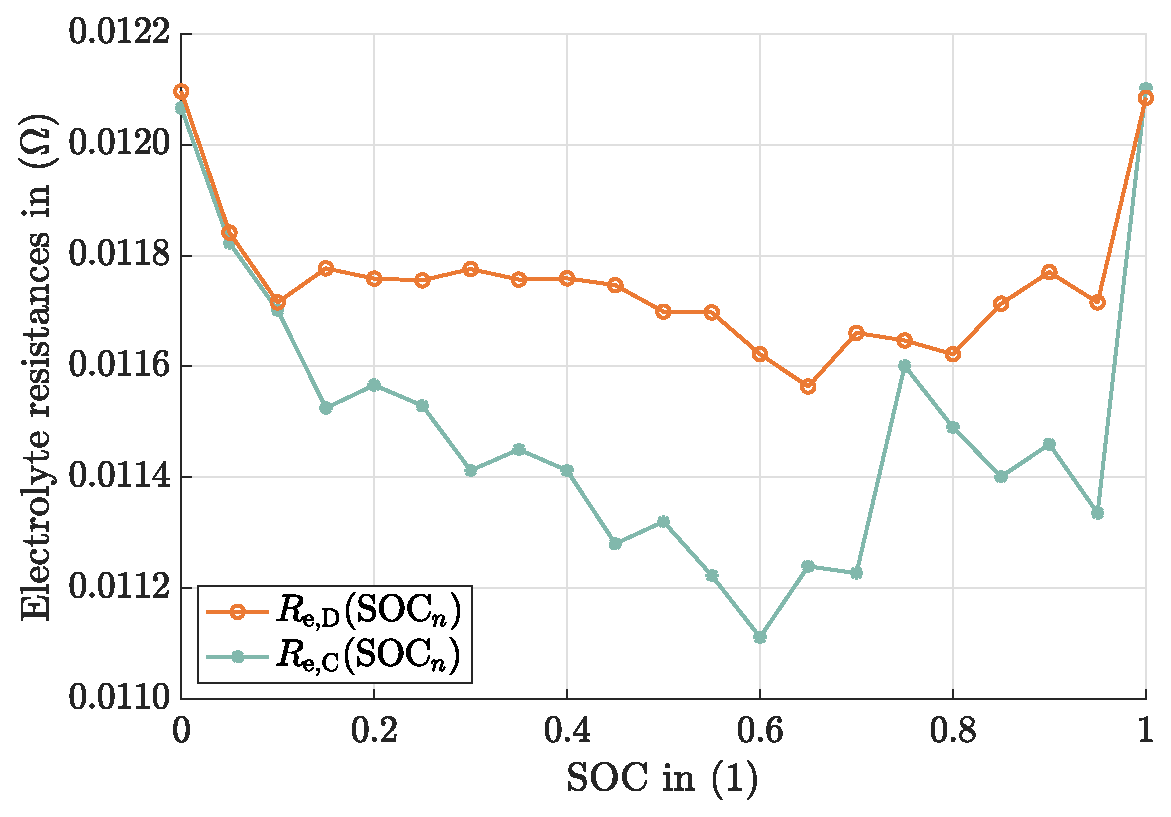
\includegraphics[width = 0.67\textwidth]{image_electrolyte_resistances_matlab.eps}
  	\caption{Electrolyte resistances $R_\mathrm{e,D}(\mathrm{SOC}_n)$ and $R_\mathrm{e,C}(\mathrm{SOC}_n)$ obtained from the discharging and charging experiment carried out on the Offgridtec Smart-Pro $12,8\mathrm{V}$ $50\mathrm{Ah}$ $\mathrm{LiFePO_4}$ battery.}
	\label{fig:image_electrolyte_resistances_matlab}
\end{figure}

Now it only remains to be shown that the assumptions for the equations (\ref{eq:battery_charge_cases}) and (\ref{current_cases}) are correct. For this purpose, the course of the charging current $I_\mathrm{C}(t)$ during the CV charging phase was measured for $\mathrm{SOC} \approx 0,99$ -- which was monitored via the Offgridtec Battery Viewer Smart app -- with Ch2 of the oscilloscope. The result can be seen in the figure \ref{fig:image_tau_b_matlab}, with the red continuous line representing the measured charging current. 
\begin{figure}[h!]
	\centering
  	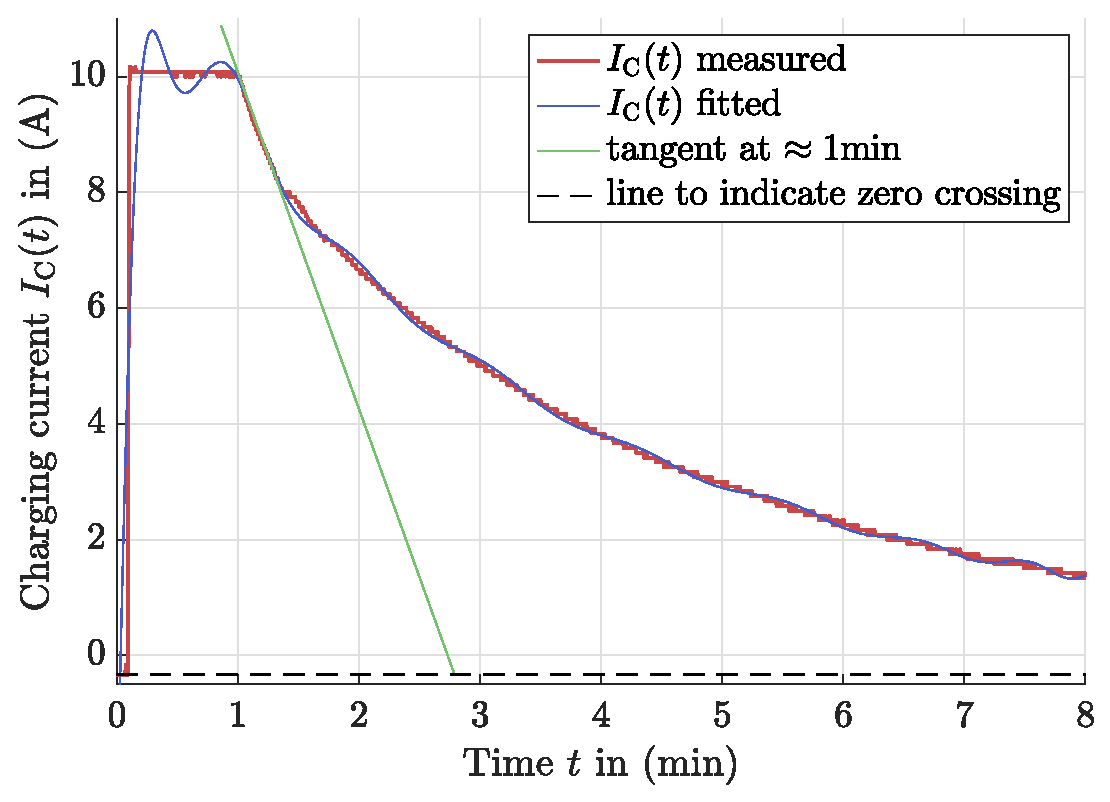
\includegraphics[width = 0.67\textwidth]{image_tau_b_matlab.eps}
  	\caption{Time course of $I_\mathrm{C}(t)$ over time during the CV charging phase of the Mean Well ENC-180-12 battery charger. The charged device was the Offgridtec Smart-Pro $12,8\mathrm{V}$ $50\mathrm{Ah}$ $\mathrm{LiFePO_4}$ battery.}
	\label{fig:image_tau_b_matlab}
\end{figure}
To prepare this measurement, the charging process of the almost fully charged battery ($\mathrm{SOC} \approx 0,99$) was switched off as soon as a decrease in the charging current was observed with Ch2 of the oscilloscope. This indicated that the battery charger was transitioning from the CC to the CV charging phase. Thereafter the battery was left to rest for 20min. The measurement was then recorded by setting the time scale of the oszilloscope to 8min, triggering Ch2 manually and continuing the charging process. First, the battery charger went into the CC charging phase and then, $t_1 = 1 \mathrm{min}$ after the start of the measurement, into the CV charging phase. No steep drop in the charging current can be seen from the recorded measurement (compare to figure \ref{fig:image_tau_b_matlab}). Thus, the described model for charging and discharging the battery from the equations (\ref{eq:battery_charge_cases}) and (\ref{current_cases}) is used for the \MATLAB simulation in the appendix \ref{sec:matlab_code}. 

As can be seen, the measured data was fitted with a polynomial function illustrated with the blue continuous line. The tangent of the polynomial fitting function, illustrated with the green continuous line, was chosen so that it runs through the point in time $t_1 = 1\mathrm{min}$ -- at which the battery charger changes from the CC to the CV charging phase. The top and bottom values of the charging current are $10,167\mathrm{A}$ and $-0,333\mathrm{A}$, with the difference between these values being the charging current in the CC charging phase $I_\mathrm{C} = 10,5\mathrm{A}$. Based on the bottom value, the black dashed line indicates the zero crossing of the measured $I_\mathrm{C}(t)$. The intersection with this line and the tangent is at $t_2 = 2,7904\mathrm{min}$. Hence, the measured time constant of the battery follows to:
\begin{equation}\label{eq:tau_battery_measured}
	\centering
	\tau_\mathrm{B} = t_2 - t_1 = 1,7904\mathrm{min}\text{.}
\end{equation}

It can be seen from the figures \ref{fig:image_dis_50}, \ref{fig:image_chg_50} and \ref{fig:image_tau_b_matlab} that the top and bottom values for the currents $I_\mathrm{D}$ and $I_\mathrm{C}$ do not quite match the values $I_\mathrm{nom}$ and $I_\mathrm{BC}$. This is likely due to the electronic loads and the battery charger. Since the behavior of these devices is only known from their data sheets, further investigations must be carried out in order to obtain more precise results. Alternatively, more professional devices that are certified for laboratory use can be used. Finally, a resistance measurement of the shunt resistor can be carried out in order to determine its exact resistance value.
